\section{Theorie}
\label{sec:Theorie}

In diesem Abschnitt soll die Funktionsweise des Operationsverstärkers (Op-Amp) und dessen Implementierung
in verschiedenen Schaltungen erklärt werden.

\subsection{Der Operationsverstärker}
\label{sec:Operationsverstaerker}
Der Operationsverstärker (Op-Amp) ist ein elektronisches Bauelement, das als Verstärker
der Differenzspannung zwischen zwei Eingängen fungiert. Ein Schaltbild eines Op-Amps ist in
\autoref{fig:opamp} dargestellt. 

\begin{figure}
    \centering
    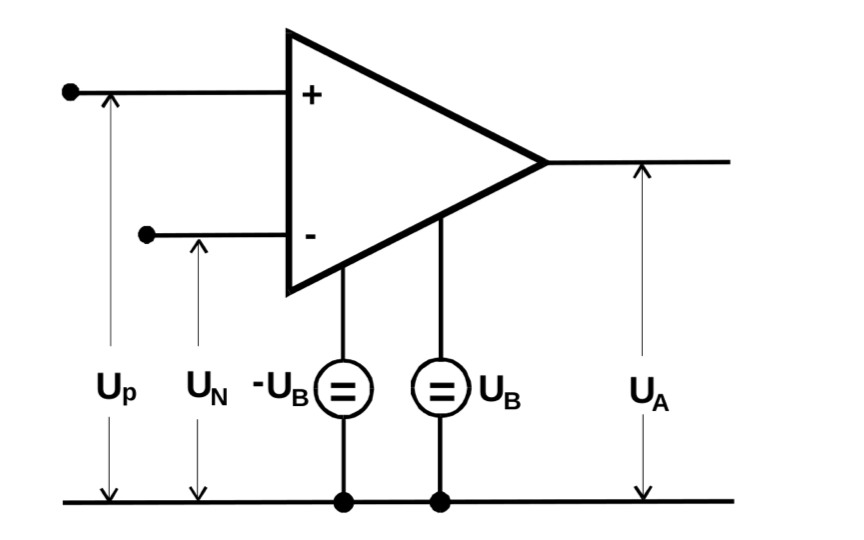
\includegraphics[width =0.48\textwidth]{figures/op-amp.png}
    \caption{Schaltbild eines Operationsverstärkers \cite{OP-Amp}.}
    \label{fig:opamp}
\end{figure}

Der Op-Amp hat zwei Eingänge, den nicht-invertierenden Eingang
($+$) und den invertierenden Eingang ($-$). Die Ausgangsspannung $U_\text{A}$ ist

\begin{equation}
    U_\text{A} = A \, (U_+ - U_-)
    \label{eq:OpAmp}
\end{equation}

mit $A$ als frequenzunabhängige Leerlaufverstärkung des Op-Amps. Die Spannungsversorgung findet über zwei 
Stromversorgungsanschlüsse statt, die hier mit $+U_\text{B}$ bzw. $-U_\text{B}$ bezeichnet sind. Diese definieren
den Bereich der Ausgangsspannung

\begin{equation}
    -U_{\text{B}} < U_{\text{A}} < U_{\text{B}}.
\end{equation}

\subsection{Der ideale Operationsverstärker}
\label{sec:IdealerOperationsverstaerker}
Der ideale Operationsverstärker ist ein theoretisches Modell, das einige Annahmen über den
Op-Amp trifft, um seine Eigenschaften zu vereinfachen. Diese Annahmen sind:
\newpage
\begin{itemize}
    \item Unendliche Leerlaufverstärkung $A \to \infty$.
    \item Unendlicher Eingangsimpedanz $Z_\text{e} \to \infty$.
    \item Null Ausgangsimpedanz $Z_\text{a} = 0$.
    \item Unendliche Bandbreite.
    \item Null Offsetspannung.
\end{itemize}

In der Praxis sind diese Annahmen nicht erfüllt, jedoch näherungsweise gültig, weshalb für die folgenden
Betrachtungen die Eigenschaften des ideale Operationsverstärker angenommen werden.

\subsection{Verschiedene Schaltungen mit Operationsverstärkern}
\label{sec:OperationsverstaerkerSchaltungen}
In diesem Abschnitt werden verschiedene Schaltungen mit Operationsverstärkern vorgestellt, welche in diesem
Versuch untersucht werden.

\subsubsection{Invertierender Verstärker}
\label{sec:InvertierenderVerstaerker}
Das Schaltbild eines invertierenden Verstärkers ist in \autoref{fig:invertierenderVerstaerker} 
dargestellt.

\begin{figure}
    \centering
    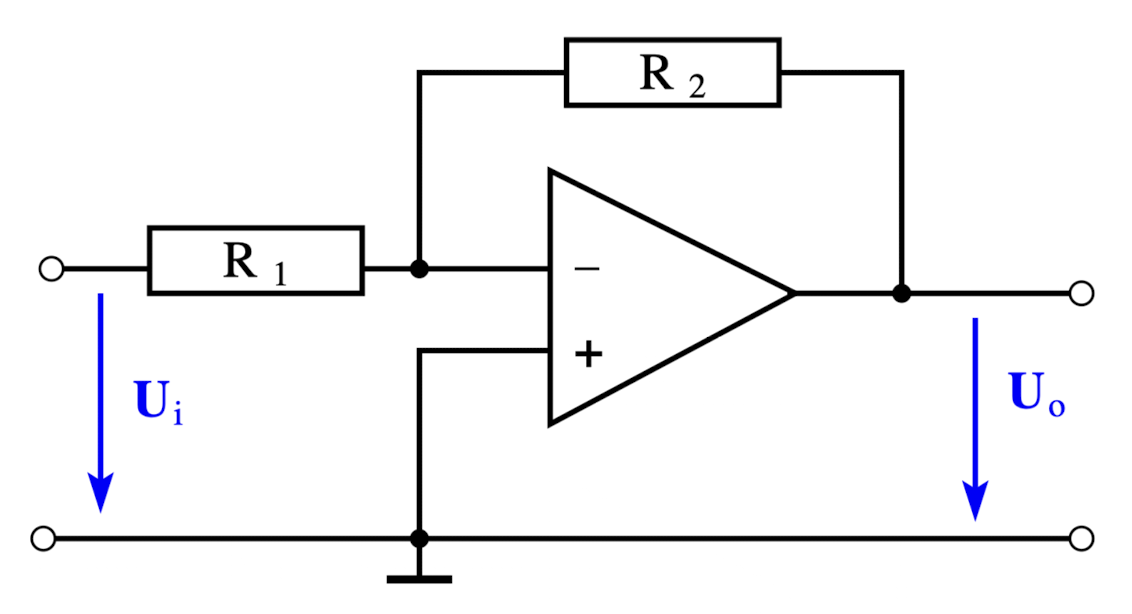
\includegraphics[width =0.48\textwidth]{figures/invertierender_verstärker.png}
    \caption{Schaltbild eines invertierenden Verstärkers \cite{Versuchsanleitung}.}
    \label{fig:invertierenderVerstaerker}
\end{figure}

Hierbei ist der nicht invertierende Eingang geerdet und der invertierende Eingang über eine Rückkopplung mit 
mit einem Widerstand mit dem Ausgang verbunden, sodass die Differenzspannung zwischen den Eingängen 
des OP-Amps verschwindet. Da das Eingangssignal $U_\text{i}$ an den invertierenden Eingang des Op-Amps 
angeschlossen ist, wird das Ausgangssignal $U_\text{o}$ invertiert. Dabei ist die Verstärkung des 
invertierenden Verstärkers durch das Verhältnis der Widerstände $R_1$ und $R_2$ gegeben

\begin{equation}
    U_\text{o} = - \frac{R_2}{R_1} \cdot U_\text{i}.
    \label{eq:invertierenderVerstaerker}
\end{equation}

\subsubsection{Integrator}
\label{sec:Integrator}
Das Schaltbild eines Integrators ist in \autoref{fig:integrator} 
dargestellt.

\begin{figure}[H]
    \centering
    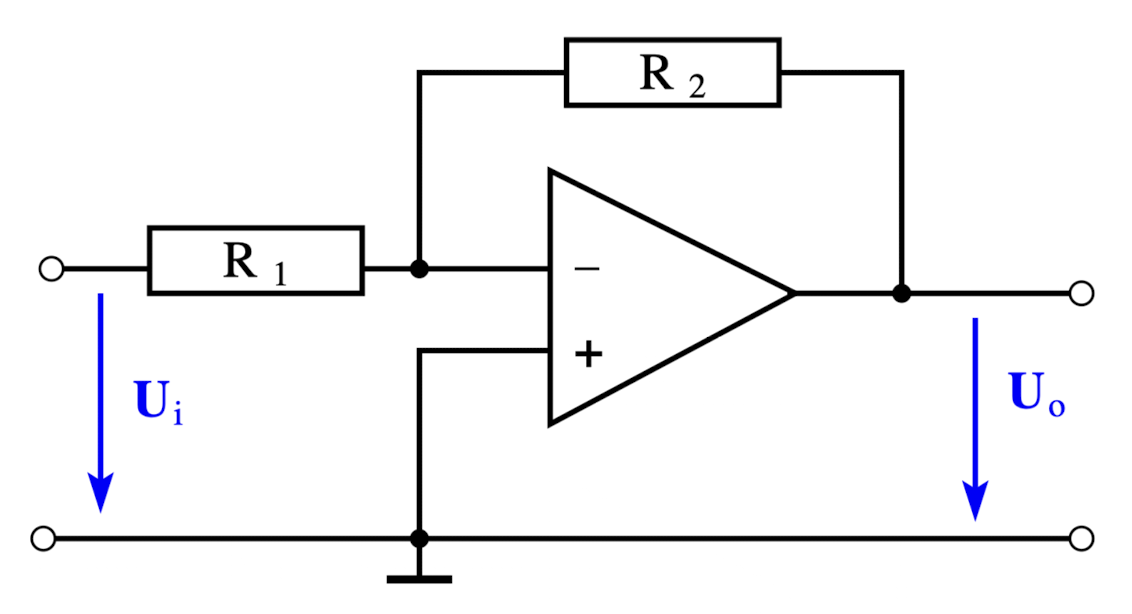
\includegraphics[width =0.48\textwidth]{figures/integrator.png}
    \caption{Schaltbild eines Integrators \cite{Versuchsanleitung}.}
    \label{fig:integrator}
\end{figure}

Hierbei ist der nicht invertierende Eingang geerdet und der invertierende Eingang über eine Rückkopplung
mit einem Kondesator mit dem Ausgang verbunden, sodass die Differenzspannung zwischen den Eingängen
des OP-Amps verschwindet. Das Ausgangssignal ist hierbei gegeben als

\begin{equation}
    U_\text{o} = - \frac{1}{R C} \, \int U_\text{i} \, \dif{t}.
    \label{eq:integrator}
\end{equation}

Angenommen ein Sinussignal $U_{\text{i}} = A \sin(2 \pi f)$ mit der Frequenz $f$ wird an den Eingang des 
Integrators angelegt, so ergibt sich als Ausgangssignal 

\begin{equation}
    U_\text{o} = - \frac{A}{2 \pi R C f} \, \cos(2 \pi f) \propto \frac{1}{f}.
    \label{eq:integratorSinus}
\end{equation}

\subsubsection{Differenzierer}
\label{sec:Differenzierer} 
Das Schaltbild eines Differenzierers ist in \autoref{fig:differenzierer}
dargestellt.

\begin{figure}
    \centering
    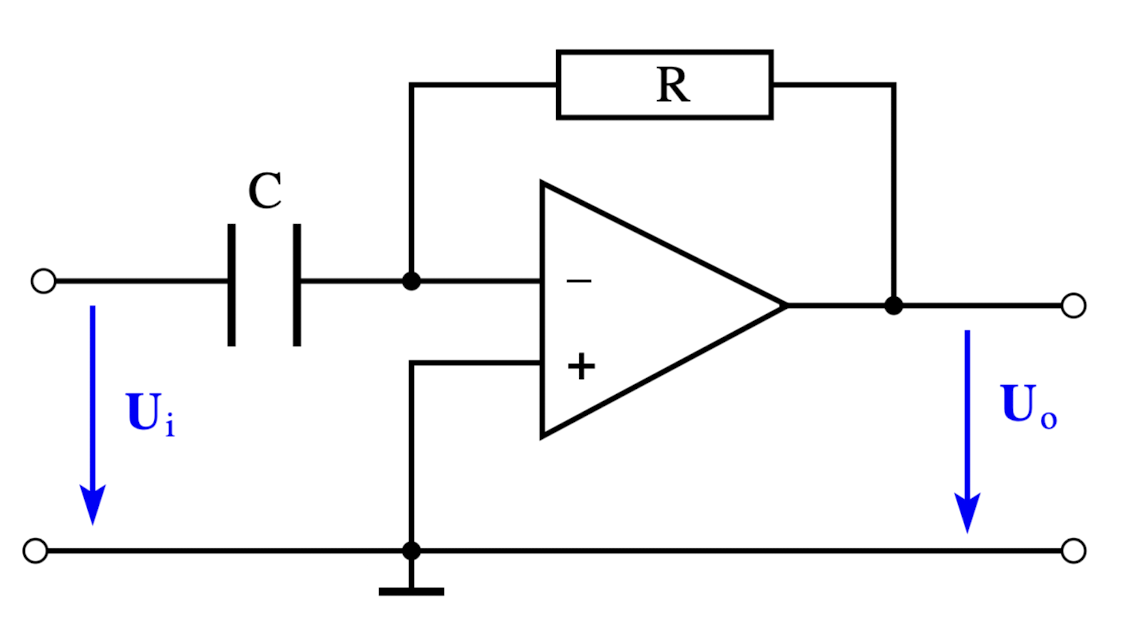
\includegraphics[width =0.48\textwidth]{figures/differenzierer.png}
    \caption{Schaltbild eines Differenzierers \cite{Versuchsanleitung}.}
    \label{fig:differenzierer}
\end{figure}

Hierbei ist der nicht invertierende Eingang geerdet und der invertierende Eingang über eine Rückkopplung
mit einem Widerstand mit dem Ausgang verbunden, sodass die Differenzspannung zwischen den Eingängen
verschwindet. Vor dem invertierenden Eingang ist ein Kondensator geschaltet. Dieser Aufbau führt dazu,
dass das Ausgangssignal $U_\text{o}$ proportional zur Ableitung des Eingangssignals $U_\text{i}$ ist

\begin{equation}
    U_\text{o} = - R C \, \frac{\dif{U_\text{i}}}{\dif{t}}.
    \label{eq:differenzierer}
\end{equation}

Angenommen ein Sinussignal $U_{\text{i}} = A \sin(2 \pi f)$ mit der Frequenz $f$ wird an den Eingang des
Differenzierers angelegt, so ergibt sich als Ausgangssignal

\begin{equation}
    U_\text{o} = - 2 A R C \pi f \, \cos(2 \pi f) \propto f.
    \label{eq:differenziererSinus}
\end{equation}

\subsubsection{Schmitt Trigger}
\label{sec:SchmittTrigger}
Das Schaltbild eines Schmitt Triggers ist in \autoref{fig:schmittTrigger}
dargestellt.

\begin{figure}[H]
    \centering
    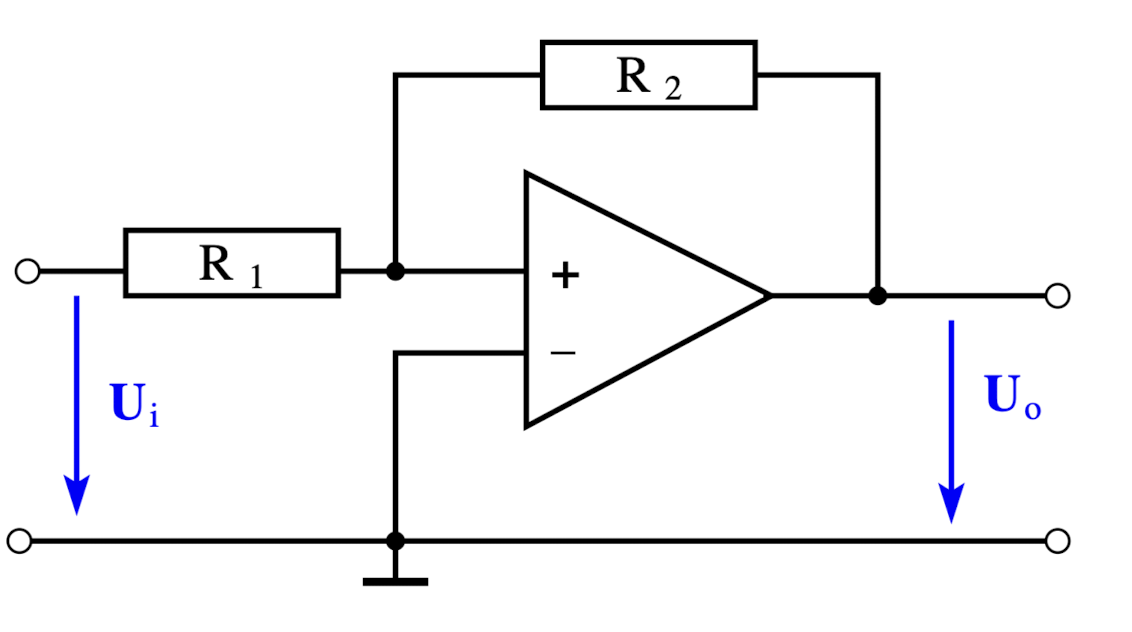
\includegraphics[width =0.48\textwidth]{figures/schmitt_trigger.png}
    \caption{Schaltbild eines Schmitt Triggers \cite{Versuchsanleitung}.}
    \label{fig:schmittTrigger}
\end{figure}

Im wesentlichen ist der Aufbau analog zum invertierenden Verstärker, jedoch findet die Rückkopplung zum
nicht invertierenden Eingang statt. Dadurch wird eine Hysterese erzeugt, die in \autoref{fig:schmittTriggerHysterese}
zu sehen ist.

\begin{figure}[H]
    \centering
    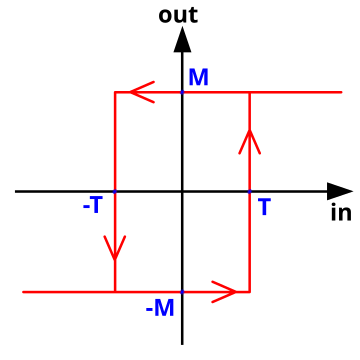
\includegraphics[width =0.48\textwidth]{figures/hysterese.png}
    \caption{Hysterese des Schmitt Triggers \cite{Schmitt-Trigger}.}
    \label{fig:schmittTriggerHysterese}
\end{figure}

Dabei ist die obere bzw. untere Schaltschwelle $\pm T$ gegeben durch

\begin{equation}
    T = \frac{R_2}{R_1} \, U_\text{B}.
    \label{eq:SchmittTriggerSchaltschwelle}
\end{equation}

Die Ausgangsspannung $U_\text{o}$ ist hierbei gegeben durch

\begin{equation}
    U_\text{o} = \begin{cases}
        U_\text{B} & \text{für } U_\text{i} > T \\
        -U_\text{B} & \text{für } U_\text{i} < -T
    \end{cases}.
\end{equation}

In allen anderen Fällen verbleibt der Schmitt Trigger in seinem aktuellen Zustand.

\subsubsection{Generator}
Das Schaltbild eines Generators ist in \autoref{fig:generator}
dargestellt.

\begin{figure}[H]
    \centering
    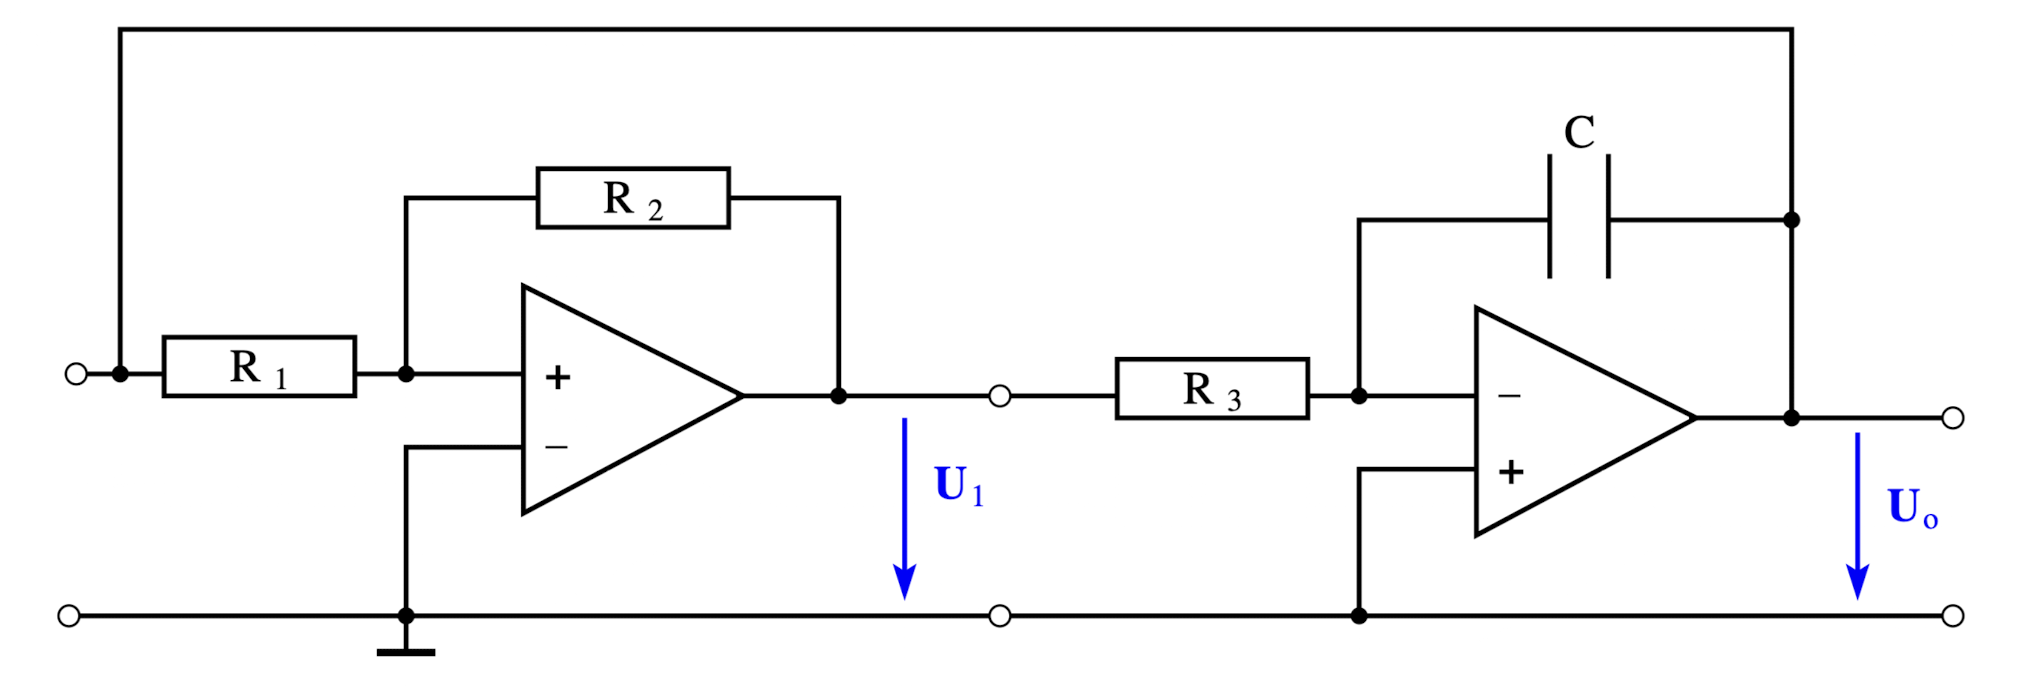
\includegraphics[width =0.8\textwidth]{figures/generator.png}
    \caption{Schaltbild eines Generators \cite{Versuchsanleitung}.}
    \label{fig:generator}
\end{figure}

Hierbei werden ein Schmitt Trigger und ein Integrator in Reihe geschaltet. Wobei der Output des
Integrators mit dem Eingang des Schmitt Triggers verbunden ist.
Durch diese Anordnung wird ein Rechtecksignal am Schmitt Trigger und ein Dreickssignal am 
Integrator mit der Frequenz 

\begin{equation}
    f = \frac{R_2}{4 C R_1 R_3}.
    \label{eq:GeneratorFrequenz}
\end{equation}

erzeugt, dessen Amplitude $A$ gegeben ist durch

\begin{equation}
    A = \frac{R_1}{R_2} \, U_\text{B}.
    \label{eq:GeneratorAmplitude}
\end{equation}

\subsubsection{Generator mit variierender Amplitude}
\label{sec:GeneratorMitVariierenderFrequenz}
Das Schaltbild eines Generators mit variierender Amplitude ist in \autoref{fig:generatorMitVariierenderAmplitude}
dargestellt.

\begin{figure}[H]
    \centering
    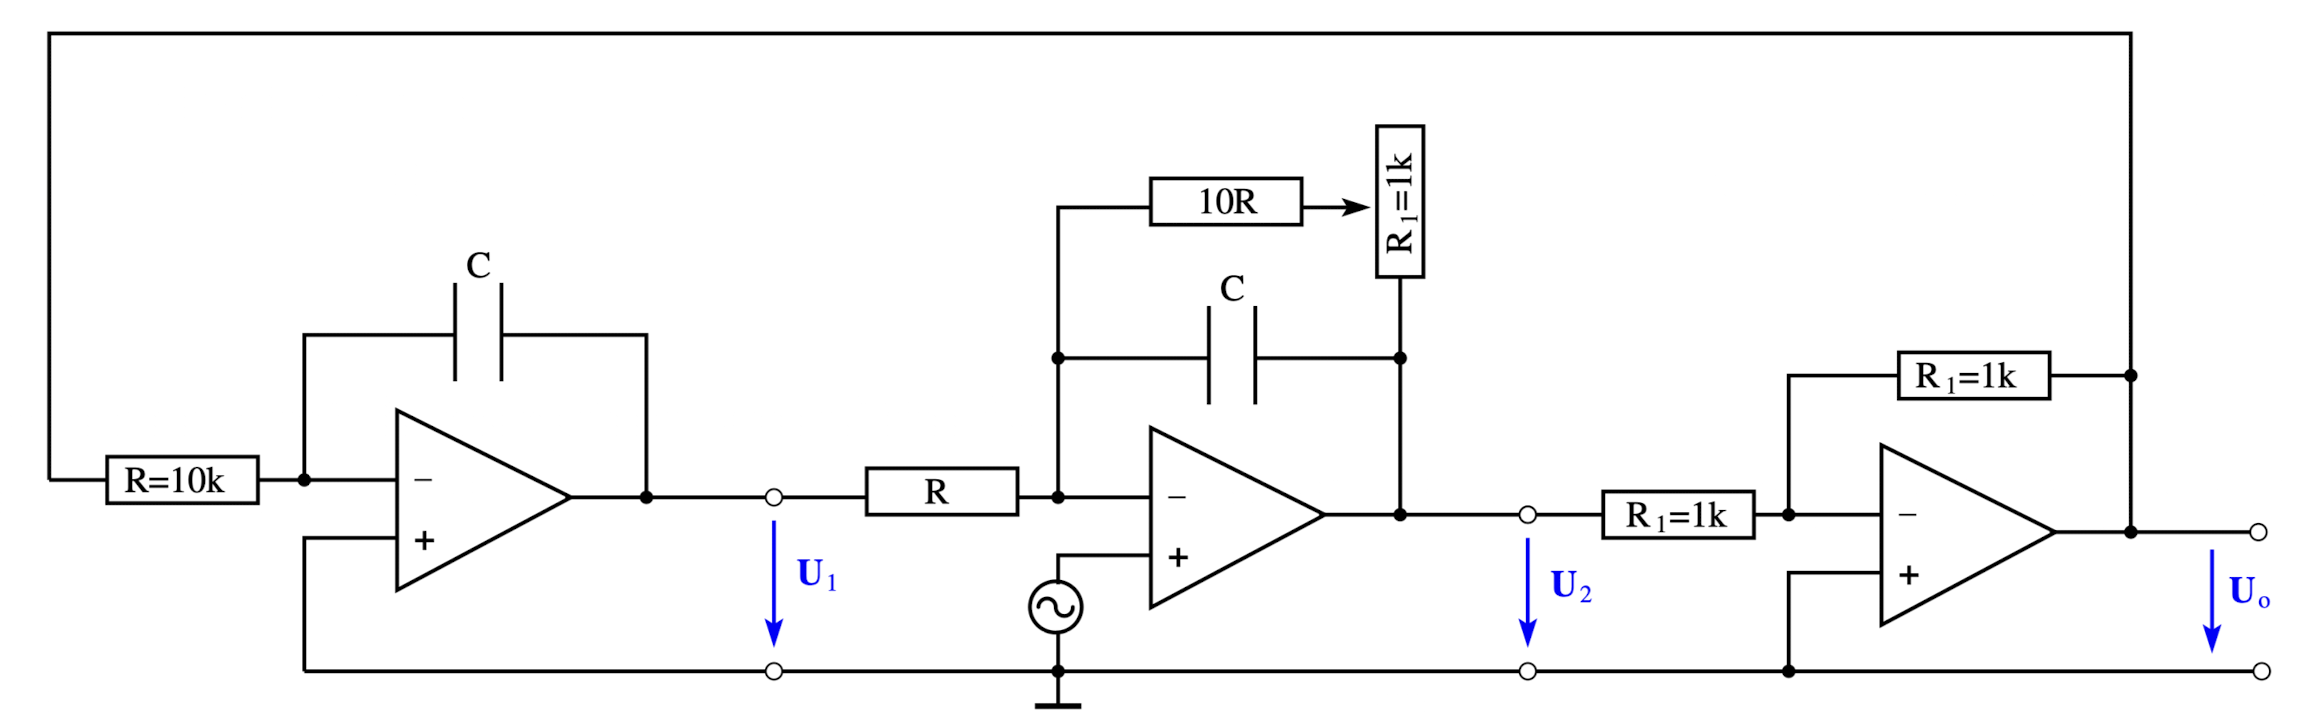
\includegraphics[width =0.8\textwidth]{figures/generator_mit_variierender_frequenz.png}
    \caption{Schaltbild eines Generators mit variierender Frequenz \cite{Versuchsanleitung}.}
    \label{fig:generatorMitVariierenderAmplitude}
\end{figure}

Es werden dafür zwei Integratoren und ein invertierender Verstärker in Reihe geschaltet. Dies führt 
dazu, dass eine gedämpfte harmonische Schwingung erzeugt wird, die durch die DGL 

\begin{equation}
    \frac{\symup{d}^2 U_\text{o}}{\dif{t^2}} - \frac{\eta}{10 RC} \, \frac{\dif{U_{\text{o}}}}{\dif{t}} + \frac{1}{R^2 C^2} \, U_{\text{o}} = 0
\end{equation}

beschrieben wird. Dabei ist $-1 \le \eta \le 1$ die Dämpfungskonstante, welche durch das Potentiometer eingestellt werden kann.
Die Lösung dieser DGL, unter der Annahme $\eta \ll 100$, ist gegeben durch

\begin{equation}
    U_\text{o}(t) = A \, \exp \l(-\frac{t}{\tau}\r) \, \sin \l(2 \pi \frac{t}{T}\r)
    \label{eq:GeneratorMitVariierenderAmplitudeLoesung}
\end{equation}

mit der Schwingungsdauer $T$ und der Zeitkonstante $\tau$, welche gegeben sind durch

\begin{equation}
    T = 2 \pi RC \quad \text{und} \quad \tau = \frac{20 RC}{\eta}.
    \label{eq:generatorMitVariierenderAmplitude}
\end{equation}